\documentclass[11pt,a4paper]{article}
\usepackage[utf8]{inputenc}
\usepackage[english]{babel}
\usepackage{graphicx}  % include graphics
\usepackage{lastpage}  % number of pages in header
% \usepackage{pgffor}    % foreach
\usepackage{color}     % for colors
\usepackage{multirow}  % multiple rows in tables
% \usepackage{latexsym}  % for \Box
\usepackage{vhistory}		% supplies us with versionhistory\usepackage[hidelinks]{hyperref}   % references in pdf file
\usepackage[section]{placeins} % keep floats where they are inserted
\usepackage{fancyhdr} % the custom header
\setlength{\headheight}{12mm}
\pagestyle{fancy}
\fancyhf{} % remove everything
\usepackage[left=2.9cm,right=2.9cm,top=2.5cm,bottom=1.5cm]{geometry} % the page margins

\title{\Huge User Manual\\[5mm]\Large SoftRF (Github astir13/SoftRF fork)\\[5mm]matching SoftRF firmware version 1.3e}
\date{2020-12-31\\[10mm]Thanks to all contributrs of the Github SoftRF Project.\\[3cm]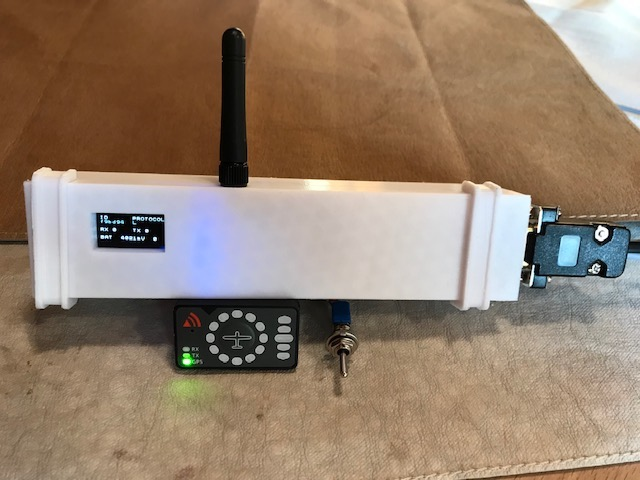
\includegraphics[scale=.4]{softrf.jpg}}
\begin{document}
% some defines
\definecolor{lightpink}{RGB}{229,172,197}
\definecolor{cadmiumred}{RGB}{230,0,38}

%titlepage
\maketitle
\newpage

% settings for the header
	\setlength{\unitlength}{1mm}
	\thicklines
	\newcommand{\graphwidth}{200}
	\newcommand{\graphheight}{11}
	\newcommand{\secondcolumnstart}{100}
	\newcommand{\secondcolumnstarttable}{\the\numexpr\secondcolumnstart - 4 mm}
	\newcommand{\bottomcalstart}{80}
	\newcommand{\bottomareastart}{60}

% the header
%\lhead{
%	\begin{tabular}{p{8cm}p{6cm}p{2.3cm}}
%	\large astir13 SoftRF & User Manual v. 1.3e rev. 0 & \hfill pg. \thepage 		(\pageref{LastPage})
%	\end{tabular}
%\begin{picture}(\graphwidth,\graphheight)
%	\put(0,\the\numexpr\graphheight){\line(1,0){\graphwidth}}
%	\put(0,\the\numexpr\graphheight - 5){\begin{tabular}{p{\the\numexpr\secondcolumnstarttable}p{6cm}}
%	\small Prepared by & \small Date/Context \\
%	\hspace{2cm}\Large Stefan Pielmeier & \hspace{2cm}\Large 2020-12-28 \\
%	\end{tabular}}
%	\put(0,\the\numexpr\graphheight - 10){\line(1,0){\graphwidth}}
%	\put(0,\the\numexpr\graphheight - 10){\line(0,1){10}}
%	\put(\secondcolumnstart,\the\numexpr\graphheight - 10){\line(0,1){10}}
%\end{picture}}
\lhead{astir13/SoftRF}
\chead{User Manual v.\/1.3e rev.\/1}
\rhead{pg. \thepage 		(\pageref{LastPage})}
\renewcommand{\headwidth}{17cm}
%\renewcommand{\headrulewidth}{0pt}

\section{Revision History}
\begin{versionhistory}
  \vhEntry{1.3e rev. 0}{2020-12-30}{astir13}{created from scratch}
  \vhEntry{1.3e rev. 1}{2020-12-31}{astir13}{editorials, added Display section, added Revision History, corrected links to fork}
\end{versionhistory}

\section{Acronyms}
\begin{description}
\item[Baidu] The GNSS deployed by China
\item[FANET] another open anti-collision protocol
\item[FLARM] The protocol used by the equipment traded by the company Flarm; the term legacy is used in the SoftRF setup and display "L", to indicate that the SoftRF does not use the Flarm protocol, as it is private and may not be used; however, the SoftRF uses a protocol, that is understood by Flarm devices and can receive Flarm transmissions as of now.
\item[GLONASS] The GNSS deployed by the Russian Federation
\item[GNSS] Global Navigation Satellite System; this can be GPS but also Glonass, Baidu or Gallileo, dependent on the chipset on the SoftRF; current SoftRF use GLONASS and GPS
\item[GPS] Global Positioning System: the GNSS deployed by the USA
\item[Gallileo] The GNSS deployed by the European Union and ESA
\item[OGN] The open glider net, see http://wiki.glidernet.org/
\item[OGNTP] another open air traffic awareness protocol
\item[RS-232] the cable-based data line protocol used for the communication between SoftRF and other cockpit equipment like Flarm LED, LX Nav/LXNavigation flight computers and smart e-varios like EOS/ERA/S-80 or S-100.
\end{description}

\section{Disclaimer}
THIS DOCUMENT IS PROVIDED "AS IS", WITHOUT WARRANTY OF ANY KIND, EXPRESS OR IMPLIED, INCLUDING BUT NOT LIMITED TO THE WARRANTIES OF MERCHANTABILITY, FITNESS FOR A PARTICULAR PURPOSE AND NONINFRINGEMENT. IN NO EVENT SHALL THE AUTHORS OR COPYRIGHT HOLDERS BE LIABLE FOR ANY CLAIM, DAMAGES OR OTHER LIABILITY, WHETHER IN AN ACTION OF CONTRACT, TORT OR OTHERWISE, ARISING FROM, OUT OF OR IN CONNECTION WITH THE SOFTWARE OR THE USE OR OTHER DEALINGS IN THE SOFTWARE, DOCUMENTATION OR HARDWARE DESCRIBED HERE.

\section{Foreword}
The SoftRF based air traffic awareness devices use the ISM bands. The devices are good tools to aid pilot situational awareness by often giving successful information about the position, direction, vertical and horizontal speed of other aviation traffic. However, they are not to be trusted all times and in all situations. Do not trust your life to this information, and only trust your eyes for VFR flight anti-collision avoidance.

SoftRF, Flarm, FANET, OGN-Tracker, Pilot-Aware, Skytraxx use transmission and reception via the so-called ISM bands, which are used for many industrial, scientific and medical purposes. Thus, the used frequencies are not exclusively reserved for air traffic transmissions, and can be used for multiple other purposes, also on board of aircrafts. No frequency coordination/licensing is provided by the authorities in most countries, which is very convenient, but there also is no protection against interference from other equipment.

\begin{center}
\fbox{\parbox{12cm}{As a consequence of potential interference from other equipment using the same frequency bands, reception in your own installation or the installation in other planes can be impaired, leading to potential "ghost" traffic, or (worse) masking existing traffic away, i.e. "hiding" other traffic.}}
\end{center}

Therefore, you should never trust such installations, nor the fact that you can detect all other planes in your vicinity using these tools. Additionally, commercial planes and motorplanes rarely use these protocols, and there is no legal carrige requirement for such equipment.

The above statements are not true for certified Mode-S transponders and TCAS equipment. Air transponders operate on reserved frequencies, may only be operated when certified and properly tested, with about 1000 times higher transmit power, and are proved to work efficiently and effectively for sailplanes, small aeroplanes and commercial planes of all sizes. In the eyes of the author, certified transponder based communication is the future of air anti-collision for all segments, but in some countries you may not be allowed such equipment in small areoplanes, drones, ultralights, and so on. So the ISM band based air traffic awareness equipment might have a long future ahead.

A note on the protocol: While Flarm is the most used protocol, it is advised to consider using the other protocols like OGN-TP because they are open source. Flarm will, thanks to the Open Glider Net initiative, not change protocol anymore, because most pilots highly rely on the existence of the open glider network to track their planes safely throughout each journey. If Flarm would change the protocol one day, remember that you can change your SoftRF to use e.g. OGN-TP through the settings menu very easily, and all open glider Net trackers would be able to "see" your plane in real time again.

\section{Basics about SoftRF}
The SoftRF main purpose is to transmit anti-collision data to other devices. In order to do so, it finds information about the own aircraft and packages it into a protocol, which then is transmitted through the SoftRF antenna on UHF ISM band frequencies.

Following data is transmitted (example from legacy protocol (Flarm v6):
\begin{itemize}
\item your position (latitude and longitude),
\item the GPS status,
\item horizontal speed (speed over ground),
\item heading (over ground from GNSS),
\item vertical speed (climb or sink rate),
\item your identification,
\item the type of aircraft,
\item stealth mode (for competitions),
\item do not track information (opt-out from OGN).
\end{itemize}

The other purpose is to receive such transmissions from other aircrafts around you and to provide this information to your other cockpit devices to issue alerts and situational awareness. Other devices can be:

\begin{itemize}
\item Android tablet or phone with XCSoar App installed
\item Flarm LED
\item LXNavigation ERA/EOS 80 devices
\item LXNav S80/100 devices
\item larger Flight computer series from LXNavigation and LXNav, or self-built
\end{itemize}

From the point in time when the SoftRF has successful reception from GNSS, it is transmitting status and all received information over following interfaces if configured correctly:
\begin{itemize}
\item Bluetooth (used for mobile phone/tablet Apps like XCSoar)
\item NMEA cable based output (RS-232) at a speed of 38400 baud
\end{itemize}

\section{Installation}
The SoftRF has to be built into a stable case, secured against overheating, examples can be seen at https://github.com/lyusupov/SoftRF/tree/master/case.

For running the astir13 fork of the SoftRF firmware, some hardware additions are required that are described in the Wiki found at https://github.com/astir13/SoftRF/wiki.

\subsection{Mechanical}
Fasten the SoftRF case and all wirings tightly with other equipment behind the instrument cluster, i.e. using wire straps. As a rule of thumb, an installation shall be able to handle +/-10G, so if your SoftRF weights 200g, the installation shall sustain a 20N force, applied at the SoftRF in each direction.

The optional FlarmLED display shall be mounted securely into the instrument panel using screws, because the supplied adhesive tape is not sufficient, follow the instructions of the producer.

\begin{center}
\fbox{\parbox{12cm}{No mechanical installations may limit or change existing mechanical functions of the aircraft.}}
\end{center}

\subsection{SoftRF Antenna}
The golden SMA female connector of the SoftRF has to be connected to a matching SMA male connector leading the RF signal to the SoftRF antenna resonating in the band of your SoftRF's transmissions. If your SoftRF is deployed in the European Union, the frequency is $868.2$MHz, and the antenna shall be resonant on this frequency. You can mount the antenna directly onto the SoftRF case or connect the antenna through a $50 \Omega$ RF cable such as RG174 for lenghts $< 1$m. For cable lengths above 1m, good results can be achived using e.g. BELDEN RF 200 cable which at many places can be bought already fully configured with SMA connectors attached.

A well-proven design is a so-called ground plane antenna on top of the instrument cluster cover, like shown in Figure \ref{groundplane}.

\begin{figure}[h]
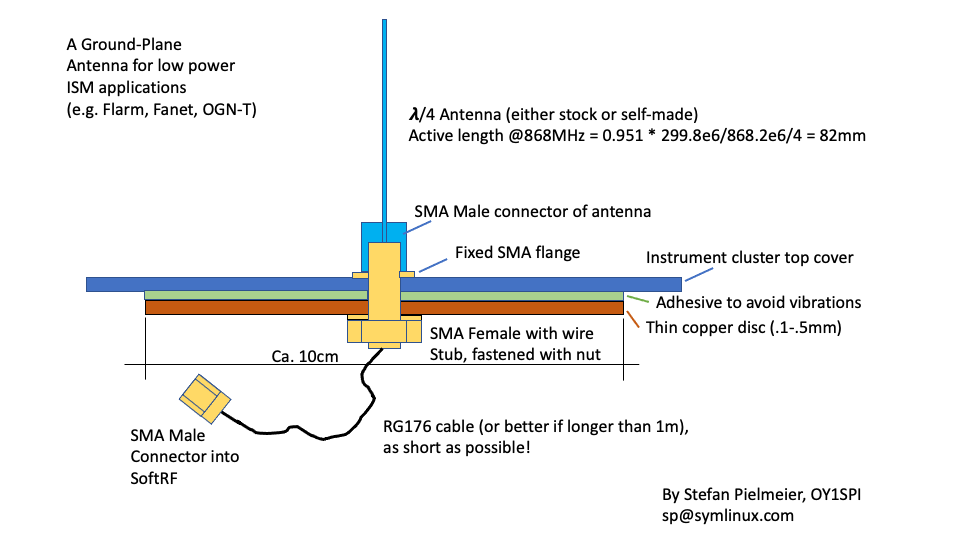
\includegraphics[scale=.5]{gp-antenna.png}
\caption{Example ground plane antenna construction that can be used for the SoftRF}\label{groundplane}
\end{figure}\FloatBarrier

Beware that there are many antennas out there that say they are Flarm compatible, but they might actually not be resonant at the required frequency. Before use, it might be relevant to test your antenna with an antenna tester to be sure it is resonant at the right frequencies. Suitable Antenna testers (e.g. Nano VNA from aliexpress) are owned by radio nerds like Amateur Radio girls and guys, find one to help you if you don't know anything about antennas, because this is an important part of achieving a good transmission range.

\subsection{GNSS Antenna}
The SoftRF needs a valid 3D position from a global navigation satellite system (GNSS), e.g. GPS or GLONASS, to define timing and the own aircraft's

\begin{itemize}
\item position,
\item horizontal speed (speed over ground),
\item vertical speed (climb or decend), and
\item heading.
\end{itemize}

The GNSS antenna is integrated into the SoftRF case's top, just in the middle, see Figure \ref{fig_gnss_ant}. Therefore, the case shall be mounted with the SoftRF display to the side and the SoftRF golden antenna plug to the top, as close as possible to the instrument cluster top cover as possible. No metal parts shall obstruct the GNSS reception field above the SoftRF middle section, otherwise GNSS reception might be impaired. 

\begin{figure}[h]
\centering
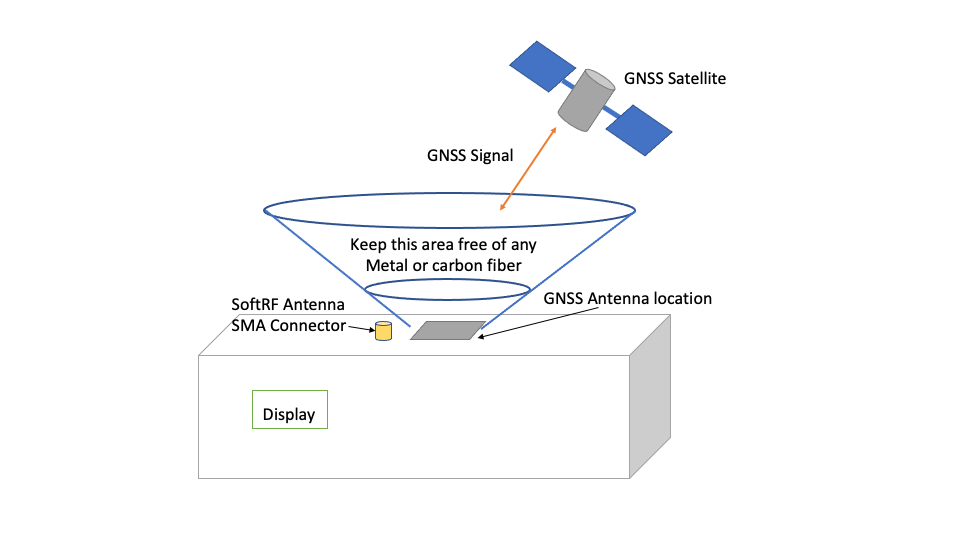
\includegraphics[scale=.5]{gnss_antenna.png}
\caption{GNSS Antenna location inside the SoftRF case}\label{fig_gnss_ant}
\end{figure}

Check for stable  GNSS reception during a test flight, ideally by using a Flarm LED, which is showing stable GNSS reception by a stady "GPS" LED in the lower left corner of the display, see Figure \ref{flarm_led}.

\begin{figure}[h]
\centering
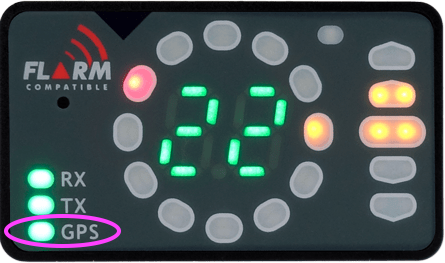
\includegraphics[scale=.4]{lxnav_flarm_led_display.png}
\caption{LXNav FLARM LED Display as an expample, notice the steady "GPS" labelled LED}\label{flarm_led}
\end{figure}

In case your GNSS reception is not stable, consider to place the SoftRF better or to modify the SoftRF to allow for an external GNSS antenna, which is totally feasible.

\FloatBarrier

\subsection{Electrical Connections}
All electrical connections are accessible through a single 9-pin D-sub connector, which is placed on the right side of the SoftRF chassis. Figure \ref{d-sub-9} shows the female connector that is part of delivery, but may be modified according to installation needs.

\begin{figure}[h]
\centering
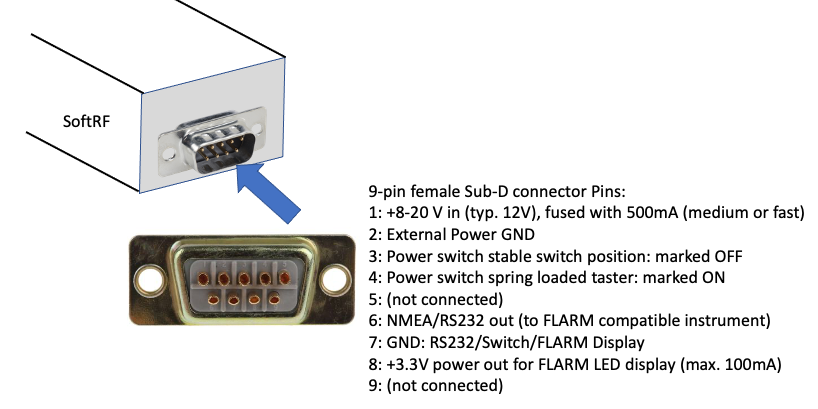
\includegraphics[scale=.5]{d-sub-9.png}
\caption{D-Sub 9 connector and pin usage}\label{d-sub-9}
\end{figure}\FloatBarrier

\subsubsection{Electrical power supply}
Electrical Power to the SoftRF is supplied to an internal power supply that operates with input voltages of 8 - 20V, supplying all internal SoftRF circuits, and the external Flarm LED display.

The Power is supplied through following of the D-Sub 9 Connector pins:

\begin{itemize}
\item Pin 1: + 8-20V = external battery "+"
\item Pin 2: Ground = external battery "-"
\end{itemize}

\begin{center}\fbox{\parbox{12cm}{The power connection shall include a blow fuse in the positive power cord, with a "M 500mA" fuse value to ensure that a shortcut failure in the SoftRF will blow the fuse.}}\end{center}

All power supply cabling behind the fuse has to be sized at least AWG30 ($0.05 {\rm mm}^2$) to ensure to blowing the fuse in case of a shortcut. It is recommended to use AWG 20 cabling for power connections in general. Cabling between the battery and the fuse has to be strong enough to blow the battery fuse, which is dependent on your the existing installation. For advice on cable sizes for certain currents, refer to FAA Advisory Circular AC 43.13-2B.

Make the fuse accessible for the pilot during flight in case the SoftRF firmware behaves unexpected, the pilot can be sure to take all power from the SoftRF.

Label the fuse in the cockpit clearly for the pilot to identify the fuse and the function, i.e. with a label called "Flarm 0.5A(M)".

To reduce the risk of interference with other equipment, all power cabling shall:
\begin{itemize}
\item be paired as close as possible together, i.e. the "+" and "-" cord shall be guided together tightly or as one double cable,
\item be distanced as far away as possible from the magnetic compass,
\item be distanced as far away as possible from the VHF radio and its cabling.
\end{itemize}

\subsubsection{NMEA out, Flarm LED}
The SoftRF D-sub 9 connector provides a RS-232 interface, that can be connected to compatible equipment.

Following NMEA sentences are implemented to be provided to external equipment:

\begin{itemize}
\item PFLAV
\item PFLAE
\item PFLAC
\item PGRMZ
\item PFLAA
\item PFLAU
\end{itemize}

These should be enough to sufficiently show: own status, closest other traffic (for alerting), most important other traffic around you.

To use this interface connect following D-Sub-9 connector pins with your equipment:
\begin{itemize}
\item Pin 6: NMEA out signal (RS-232)
\item Pin 7: signal ground
\item Pin 8: +3.3V for small (max. 100mA) devices like the Flarm LED
\end{itemize}

The author does not give any guarantee for correctness, it is the responsibility of the person integrating the equipment to ensure that voltage levels between equipment is compatible. Short-cutting the 3.3V supply might damage the SoftRF, exchanging the power line polarity might damage the Flarm LED.

The NMEA out baud rate is 38400 baud, this needs to be adjusted in the connected equipment in order to ensure proper operation.

The SoftRF does not listen to any NMEA input data, you cannot configure or update the SoftRF via NMEA, but only thogh WIFI, see section \ref{parameters}.

\subsubsection{Power Switch}
In order to conveniently integrate the SoftRF in a sailplane installation without the need to physically access the SoftRF itself, a special power switch function is integrated into the SoftRF. 

The recommended power switch is of type ON-OFF-(ON), a "Myiama Parts MS500D" or similar. It does not switch currents, the actual switching is done by the power control chip inside the SoftRF. The switch has 3 positions and is connected as follows:

\begin{itemize}
\item Stable middle position: no action; connect to D-Sub-9 Pin 7 (GND)
\item Stable OFF position: device shall be OFF; connect to D-Sub-9 Pin 3
\item unstable/spring loaded ON position: device ON command; connect to D-Sub-9 Pin 4
\end{itemize}

The function of the power switch is described in section \ref{usage_power}.

\subsection{Parameters}\label{parameters}
At least for the first 10 minutes after power-on, the SoftRF creates a WIFI network named "SoftRF-AABBCC", where AABBCC is the SoftRF Device ID of your SoftRF, find it on a label that is found on the SoftRF, and on the small display of the SoftRF.

The password for this WIFI network is 12345678, it cannot be changed.

Connect to this WIFI using your mobile phone or PC, and type following URL into your favourite web browser "http://192.168.111.1/" and hit "Enter".

This shows you a status page similar to Figure \ref{status}:

\begin{figure}[h]
\centering
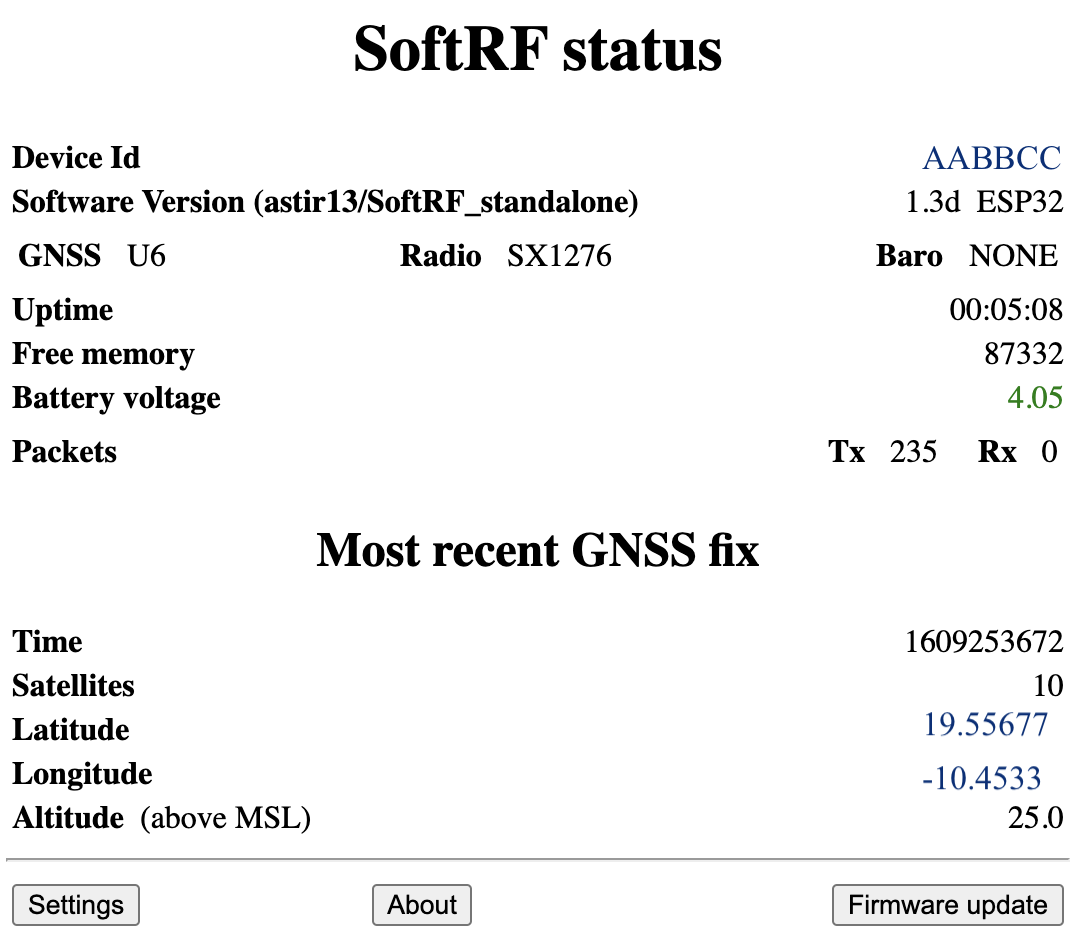
\includegraphics[scale=.6]{status.png}
\caption{Status page in web browser at http://192.168.111.1}\label{status}
\end{figure}\FloatBarrier

This example shows a status where there are 10 GNSS satellites found, and lat/long is provided. The device ID that will be found on e.g. http://glidertracker.org is shown as "AABBCC".

When pressing the "Settings" button in the lower left area of the screen, another screen is shown, see Figure \ref{settings}.

\begin{figure}[h]
\centering
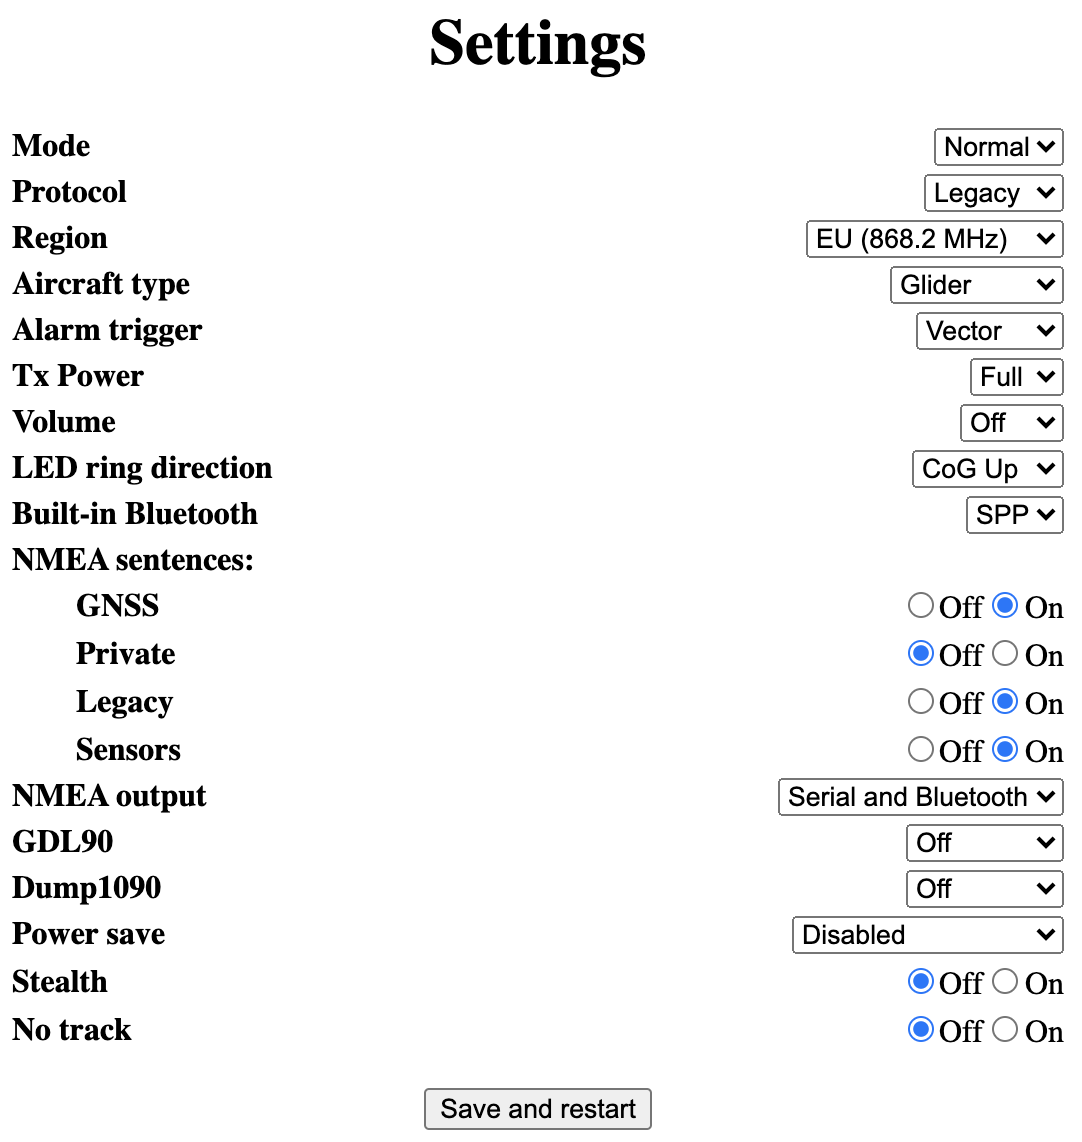
\includegraphics[scale=.6]{settings.png}
\caption{Settings page in web browser at http://192.168.111.1/settings}\label{settings}
\end{figure}\FloatBarrier

All settings can be changed. To provide proper operation for sailplane usage, however, only following settings shall be changed to stay on the safe side:

\begin{itemize}
\item Protocol: choose "legacy" if you want to see other Flarm devices and if you want to be seen by other Flarm devices; use OGN-TP, if you just want to be tracked by the open glider network database, i.e. on http://glidertracker.org. Only use other protocols than "legacy" if you really know what you do and what the consequences are.
\item Region: select the right one, to ensure you use a legal frequency. This might have to be changed when you travel with your glider to e.g. Russian Federation from European Union. However, you can not freely choose all frequencies as your SoftRF is born in a certain frequency band, which limits your choices around that band.
\item Aircraft Type: choose according to your aircraft type
\item Alarm Trigger: "Vector" is an intelligent way to create alerts from course over ground and speed to issue alerts if an impact is expected in 19 seconds or sooner; "Distance" creates alerts for the closest received traffic that is closer than 1000m horizontal and 300m vertical, with different levels of urgency, highest urgency level with distance < 400m;
\item Tx Power: Inside the EU, "EU" should always be used which limits TX power to 25mW (14 dBm) at the Antenna, which is the maximum in the EU; FULL is 17 dBm, and LOW is 2 dBm, these might be chosen at other places;
\item Built-in bluetooth: "SPP" shall be chosen if this manual shall apply
\item NMEA output: "Serial and Bluetooth" ensures you can use a Flarm LED or other cabled device and a bluetooth device to run e.g. XCSoar App at the same time. If you only want one or the other, choose accordingly, but remember that other pilots might expect bluetooth to work.
\item Power Save: "WIFI Off 10 min." allows you to disable WIFI after 10 minutes from power-up. This can be advisable to ensure no one can temper with your settings when waiting for the towplane, etc. and it safes some power.
\item Stealth: "On" informs other aircraft and ground receivers (open glider net), that you are in stealth mode, i.e. used at centralized competitions, where you do not want to share your position and climb rate with other gliders, but you want to have awareness of collision relevant traffic around you, see also http://wiki.glidernet.org/opt-in-opt-out.
\item No Track: "On" informs the open glider network to hide your position and track (OGN opt-out), including search and rescue, see also http://wiki.glidernet.org/opt-in-opt-out.
\end{itemize}

When having changed any of these settings, press the "Save and restart" button in the bottom of the page and wait approximately 20 seconds for the device to be restarted before reconnecting to the SoftRF WIFI with your PC or mobile to check if the status is ok and to {\em verify your settings} are really changed.

Always test the new settings in the concrete installation scenario before using the SoftRF equipment in flight.

\subsection{Internal Battery}\label{battery}
If not yet installed, install a "protected" LiIon 18650 battery into your SoftRF. The battery is needed to stabilize the power supply for the SoftRF itself and the optional external Flarm LED.\\

It is highly recommended for fire hazard reasons to apply a high quality 18650 Li-Ion 3.6/3.7V cell from your country that has a battery management system protection included. Buying in your country also ensures all environmental and legal battery requirements are fulfilled. One example for a very suitable type of battery is the NITECORE NL1826R 2600mAh.\\

Be aware:

\begin{itemize}
\item Never install a Li-Ion battery that is damaged, old, was overheated, is below $-15$ degrees Celsius, or is disformed in any way from its normal size.
\item Never install a Li-Ion battery that has no battery management system integrated.
\item the SoftRF has a Li-Ion battery charging controller, so there shouldn't be any danger from over- or undercharging, but safe is better than sorry, so use a battery management system battery for double protection, as should be normal in an aeroplane.
\item do not use other chemical types of batteries, as the SoftRF assumes a Li-Ion battery to be used.
\item Li-Ion batteries with battery management system typically are the ones used in devices where batteries are user-replaceable, as is the case for LED lamps and e-cigarettes.
\end{itemize}

\subsection{setup in OGN Database}
You want to be a part of the open glider net community to allow others to see your SoftRF tracking in e.g. http://glidertracker.org, then go to http://wiki.glidernet.org/ddb and register your glider there with the "Device ID" shown in the WIFI Status page, see section \ref{parameters}.

\subsection{Sticker in Cockpit}
Place the sticker shown in Figure \ref{sticker} in the cockpit for pilots to be able to find documentation about the use of the SoftRF. Simply print this page on paper, cut it out, write the Device ID, then laminate and apply in the cockpit.

\begin{figure}[h]
   \centering
	\setlength{\unitlength}{1mm}
	\thicklines
	\renewcommand{\graphwidth}{75}
	\renewcommand{\graphheight}{30}
   \begin{picture}(\graphwidth,\graphheight)
		\put(0,\the\numexpr\graphheight){\line(1,0){\graphwidth}}
		\put(0,0){\line(1,0){\graphwidth}}
		\put(0,\the\numexpr\graphheight){\line(0,-1){\graphheight}}
		\put(\graphwidth,\the\numexpr\graphheight){\line(0,-1){\graphheight}}
		\put(1,1){
\includegraphics[scale=.4]{pilot-help.png}}
		\put(30,25){astir13/SoftRF}
		\put(30,20){T-Beam Modem HW 1.1}
		\put(30,15){astir13/SoftRF HW 1.0}
		\put(30,8){DeviceID}
		\put(30,3){\color{cadmiumred}$\leftarrow$ scan QR for usage}
%		\put(0,\the\numexpr\graphheight - 5){\begin{tabular}{p{\the\numexpr\secondcolumnstarttable}p{6cm}}
%		\small Prepared by & \small Date/Context \\
%		\hspace{2cm}\Large Stefan Pielmeier & \hspace{2cm}\Large 2020-12-28 \\
%		\end{tabular}}
%		\put(0,\the\numexpr\graphheight - 10){\line(1,0){\graphwidth}}
%		\put(0,\the\numexpr\graphheight - 10){\line(0,1){10}}
%		\put(\secondcolumnstart,\the\numexpr\graphheight - 10){\line(0,1){10}}
  \end{picture}
  \caption{Cockpit sticker with QR code leading to online documentation}\label{sticker}
\end{figure}\FloatBarrier

\subsection{Test}\label{test}
After installation, you shall test the installed SoftRF by placing your aircraft outside, sitting inside with a closed canopy and starting all your cockpit equipment including the SoftRF. Please observe in this ground test positively that:

\begin{itemize}
\item total power consumption does not exceed the design maxima for your aircraft (measure current, consult documentation),
\item all aircraft equipment operates as usual before the installation of the SoftRF,
\item that the VHF Radio does not produce a noise that could result from interference from the SoftRF,
\item a radio check via the VHF radio is positive with good readability from a test station,
\item your magnetic compass shows the correct direction (compensation might be necessary if power supply wires pass close to the compass),
\item the SoftRF has turned on (see the display),
\item the SoftRF has GPS reception (see the status page, refer to \ref{parameters}),
\item the SoftRF transmits (see the status page transmit counter, refer to \ref{parameters}),
\item (optional) the SoftRF is registered at OGN DB with the correct Device ID (shown in the display),
\item (optional) the SoftRF is received by a nearby OGN receiver (if there is one), verify on a glider tracker web page such as http://glidertracker.org; the heading of the SoftRF might be wrong, as the GNSS cannot determine a meaningful heading without movement,
\item the SoftRF is received by another nearby SoftRF receiver (or FLARM, ideally with a display or XCSoar to verify your identification and location),
\item the SoftRF receives other SoftRF transmitters using the same protocol,
\item auto-power off after 10 minutes if you shut down the external power of the SoftRF and when the aircraft does not move.
\end{itemize}

After a successful ground test, perform a flight test or let an experienced person perform a flight test with all existing and the new equipment switched on to positively confirm that:

\begin{itemize}
\item the SoftRF can be received by other aircraft equipped with compatible equipment (ask your friends)
\item the SoftRF receives the other aircrafts: e.g. on the XCSoar moving map app
\item the SoftRF is received by the nearby OGN Receiver, to check this, log onto http://glidertracker.org, select your plane by clicking on it, and choose from the Settings "track"= 12h and "Select"=12h, this should show your whole flight, dependent also on the altitude of your flight and the location of OGN receivers;
\item after a long flight where you covered different OGN receiver areas, check out your SoftRF range as received by the OGN network using this tool: https://ktrax.kisstech.ch/flarm-liverange/.
\item keep this range analysis for later reference (yearly check).
\end{itemize}

If you are encountering unexpected results in these tests, check the installation and antenna characteristics.

Noise in the VHF radio can be removed by following steps:
\begin{itemize}
\item identifying the source of the noise: keep your radio on with squelch off, to hear the noise, switch off the other devices one by one until the noise suddenly vanishes; switch on the last device again to confirm that it is the noise generator;
\item now use a EMI Suppression Toroidal Ferrite (e.g. 3W800 from Würth), that ranges up to VHF Air Radio frequencies and wind the power supply cabling of the noise generating device 2-3 times through the ferrite (both ground and positive), as close as possible to the casing of the noisy device,
\item ensure the 2 cables ground and positive are both following each other closely until the source of power,
\item if not effective, apply the ferrite to other cables leaving the device; especially SDCard reader cables, GPS antenna cables are earlier seen to carry noise into other instruments.
\end{itemize}

\subsection{Legalities}
For the european union, the EASA CS STAN Issue 3 defines the CS-SC051c standard change for "the installation on of FLARM equipment in ELA2 type aircrafts", giving very good advice on the installation procedures to follow. This document highly recommends to follow that standard change regardless of your country, as it gives good advice.

Find the document at https://www.easa.europa.eu/sites/default/files/dfu/CS-STAN\%20Issue\%203.pdf

If you are placed in a country that implement EASA rules, you and your aircraft material personnel shall fill out a Form 123 (find it e.g. here: https://www.iaa.ie/publications/docs/default-source/publications/forms/airworthiness-application-forms/easa-form-123-issue-00) and refer to CS-SC051c.

\section{Usage}
During normal use, the SoftRF offers the following functions:

\begin{itemize}
\item transmission of own aircraft information to other aircrafts and ground receiver stations (OGN Receivers), using the chosen protocol (default is Legacy = compatible with Flarm v6)
\item reception of other aircraft information using the chosen protocol (default is Legacy = compatible with Flarm v6)
\item transmission of GNSS data, current own state, alerts and other aircraft information to connected devices through bluetooth and RS-232 cabling
\item charging of the internal battery to continue operation after the main power fails
\item display of status on a small internal display, for debug on ground
\end{itemize}

Some of these functions can be manipulated by the setup menu, refer to section \ref{parameters}.

\subsection{Power on/off and preflight check}\label{usage_power}
This section assumes, you have a Flarm LED device connected. For installations without Flarm LED, a specific procedure shall be prepared and handed to the pilots by the installation personnel.\\

\subsubsection{Switch ON}\label{power_on}
To switch the SoftRF ON, perform following steps:

\begin{itemize}
\item connect the battery to the aircraft, 
\item switch the main switch of the aircraft into "ON" position, to provide external power to the SoftRF,
\item {\bf press the SoftRF Power button into position "ON" and hold it there for 2 seconds, then release it to middle position},
\item observe the Flarm LED or a LED besides the SoftRF power switch turn on
\end{itemize}

Before flying with the SoftRF, check its function when outside on the airfield, at least 20 seconds after switching "ON":
\begin{itemize}
\item check that the SoftRF is having GNSS reception, the "GPS" LED on the Flarm LED device shall be permanently green and on, as shown in Figure \ref{flarm_led}
\item check that the SoftRF is transmitting by e.g. checking that the LED marked "TX" on the Flarm LED device is blinking green once per second, it is located just above the "GPS" LED;
\item if other aircrafts are around, and their SoftRF (or compatible devices) are switched on, check that you receive their signal, shown on a connected XCSoar device or by observing that the "RX" LED on the Flarm LED is blinking, it is located just above the "TX" LED;
\end{itemize}

\subsubsection{In-flight switch OFF}
To switch OFF your SoftRF in flight, i.e. because you get distracted by too many alerts during aero-tow or otherwise, just switch the SoftRF power switch into the "OFF" position and leave it there. The SoftRF will shut down after 5 seconds.

\subsubsection{Switch OFF after flight}
To switch off your SoftRF at the end of the flight:
\begin{itemize}
\item switch off the main power supply of the aircraft,
\item observe the SoftRF to continue operation for the next 10 minutes and then to show down itself automatically (this extends the life of the battery because it is not stored fully charged)
\end{itemize} 

The auto-shutoff function only happens when the GNSS measured speed is below 10kt for at least 10 minutes while external power is off.

\subsection{Power outage}
If the aircraft's main power supply fails during flight, the SoftRF will continue to operate on power provided by the internal battery. The duration of operation depends highly on the charge in the battery, but should last at least for 60 minutes with an external Flarm LED supplied as well.

\begin{center}
\fbox{\parbox{12cm}{Do not use the SoftRF as an indicator for the state of the aircraft's main power supply, as the SoftRF will change over to internal battery power if the external supply fails. The user cannot see any difference during flight.}}
\end{center}

\subsection{Display}
The SoftRF contains a little OLED display with status information, mostly for debugging. All information shown is also available through the Status page over WIFI, see \ref{parameters}.

\begin{figure}[h]
\centering
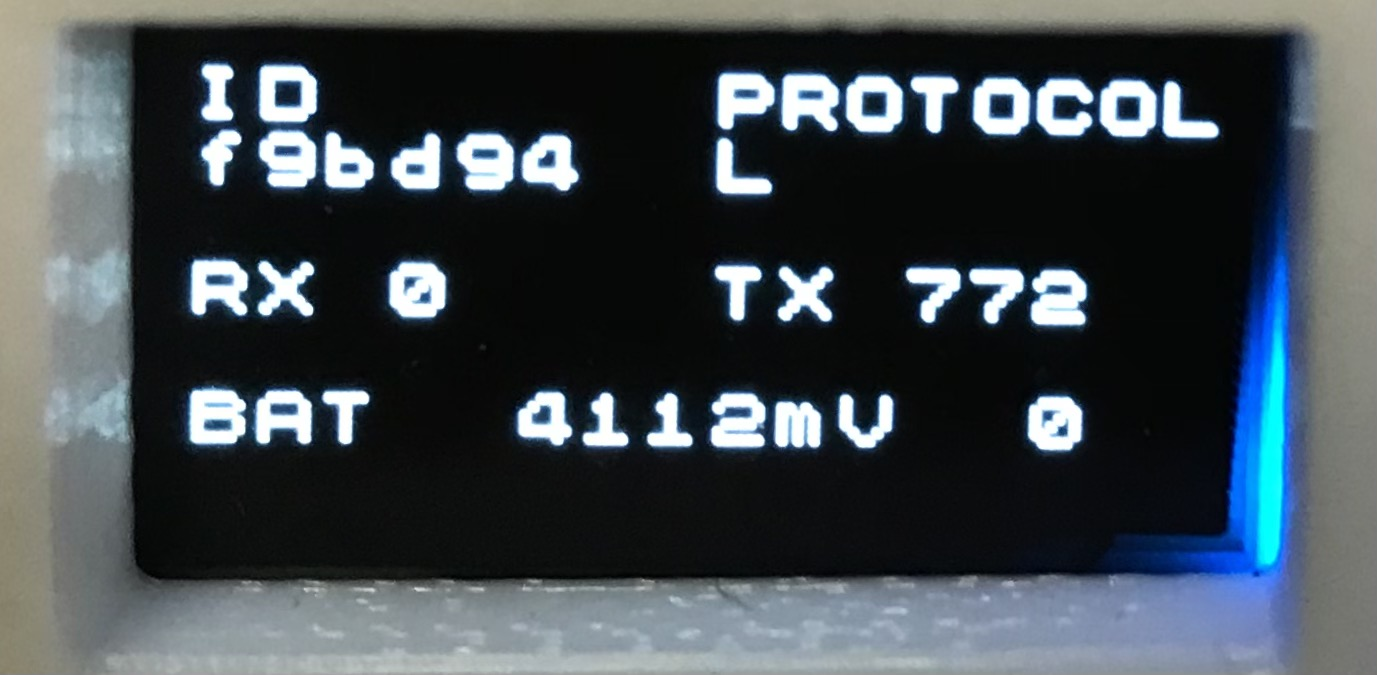
\includegraphics[scale=.1]{display.jpg}
\caption{SoftRF Display}\label{display}
\end{figure}\FloatBarrier

Figure \ref{display} shows a typical screen view of the SoftRF display with following content:

\begin{itemize}
\item top left: "ID" and below the Device ID
\item top right: "PROTOCOL" and below "L" for Legacy (= Flarm v6 compatible)
\item left middle: "RX" and to the right "0": the number of received packages from other transmitters
\item middle middle: "TX" and to the rigth "772": the number of transmitted packages, shall increase by 1 each second (roughly), when GNSS reception is working; if not incrementing, the GNSS reception might be bad (aircraft inside hangar, or GNSS antenna blocked)
\item lower left: "BAT" and to the right "4112mV" the internal battery voltage, is about 4160mV when fully charged;
\item lower right: "0" counting from "0" to "5" when in "OFF" position before the SoftRF shuts down
\end{itemize}

\subsection{Power Chip Reset}\label{power_reset}
If the operation of the power switch doesn't work as described above, you can reset the power controller chip of the SoftRF by pressing the power switch into "ON" position and hold it here for >8 seconds, then release it to middle position. Then the device is OFF. After that a short press of 2 seconds into "ON" position, it should turn on. If that does not work, check the power supply of the SoftRF, the state of the internal battery, probably best done by the personnel that installed the SoftRF in that aircraft.

\subsection{Connecting XCSoar via Bluetooth}
In order to make the widespread soaring app "XCSoar" show you other traffic around your plane on the moving map and the opftional screen "Flarm Radar", please follow following steps:

\begin{itemize}
\item enter the Android Bluetooth settings menu on your mobile device running XCSoar
\item scan for other devices
\item the list of devices should show "SoftRF-ABCDEF" where ABCDEF is the Device ID of your device (visible on the little display in the SoftRF and on a sticker visible for the pilot)
\item press on the "SoftRF-ABCDEF" device to pair the SoftRF
\item open XCSoar in flying mode
\item open the XCSoar Config/Devices menu
\item identify a unused device that says "Disabled" and select it, 
\item press the "Edit" button in the bottom,
\item for the Port, select the "SoftRF-ABCDEF" device you just paired before,
\item for the Driver, select "FLARM",
\item for thee K6Bt, select "OFF",,
\item press OK
\end{itemize}

Now the SoftRF is setup and if it currently has GNSS reception, the Devices screen should show you below your SoftRF Device a line with small text saying "GPS fix; Baro; FLARM".\\

Note: Pressing the "Monitor" button in the Device menu allows you to see the NMEA traffic that is generated by the SoftRF. This might be very useful for debugging problems.

\section{Maintenance}
As the SoftRF is not mandatory equipment, there is no mandatory maintenance required.\\

However, to maintain proper operation, it is recommended at regular intervals, not longer than 12 month since the last time, the following maintenance is to be executed.

\subsection{Range check}
If your flights during the last months have been in an area with compatible OGN receivers, and you had not opted out from OGN actively, you shall check your transmission range still is as at installation time with this tool: https://ktrax.kisstech.ch/flarm-liverange/.

\subsection{Internal Battery}\label{maint_battery}
Run an internal battery test:

\begin{itemize}
\item connect the main aircraft power supply battery,
\item switch the SoftRF "ON", see \ref{power_on},
\item open the Status page as described in section \ref{parameters},
\item let the SoftRF charge the internal battery until it reads ~4.1-4.2V in the SoftRF status page, if you have enabled WIFI power saving, you might require to read the battery voltage on the SoftRF display or restart the SoftRF to provide WIFI anew,
\item disconnect external power, take the time and observe the battery voltage to decline slowly,
\item when the SoftRF shuts down 10 minutes later (auto-power off), because the aircraft is not moving and on battery power (as described in section \ref{usage_power})
\item switch the SoftRF "ON" again, and reconnect to the status page, to read the Battery voltage: if the battery voltage is below 4.00 (Volt), the battery might need a capacity check and possibly replacement, see \ref{battery}.
\item if the battery voltage after the 10 minutes test is greater or equal 4.00 (Volt), the battery can be expected to keep up operations for at least 60 minutes when in flight
\end{itemize}

\subsection{Firmware}

\begin{itemize}
\item connect to the status page as described in section \ref{maint_battery}
\item check https://github.com/astir13/SoftRF/wiki/Updates if there is a new Software Version for your device,
\item in case there is a new firmware for your device and you decide the updates are relevant for your use, continue this list:
\item continue on a PC (Mac, Linux, Windows are ok): download the new firmware for your device from https://github.com/astir13/SoftRF/wiki/Updates (you need internet connection for that), be careful to check that the two HW Revisions match the ones on the sticker of your SoftRF (T-Beam and astir13/SoftRF HW revision)
\item disconnect from the internet WIFI,
\item connect to the SoftRF WIFI,
\item open the status page of the SoftRF,
\item click on the button "Firmware Update",
\item observe a new page opens called "Firmware update",
\item click on "Choose File" button,
\item select the downloaded file name from your Download directory, it shall end with ".bin", if you downloaded a zip file, you might need to unzip it first to get to the ".bin" file,
\item observe the filename be shown besides the "Choose File" button,
\item click on the "Update" button, to start the upload,
\item {\bf do not shut down power now!}
\item observe the update counter to count to 100, then wait for at least 3 minutes without taking power off the SoftRF,
\item in case the counter stops for more than 60 seconds without update before reaching 100: wait 60 seconds more, then perform a power chip reset (see section \ref{power_reset} and retry;
\item after above procedure, the SoftRF should restart and display the new firmware revision in the status page and on the built-in display
\item run a functional test, see section \ref{test}.

\end{itemize}

\section{Technical Data}

\subsection{Hard- and Software}
The SoftRF is open source hardware and software. Please find the SoftRF firmware and hardware descriptions at http://github.com/astir13/SoftRF.

\subsection{Transmit Spectral Purity and Power}
For T-Beam HW revision 1.1, following transmit spectrum was recorded in EU power setting, which shows very good spectral cleanness and power below the maximum allowed +14dBm:

\begin{figure}[h]
\centering
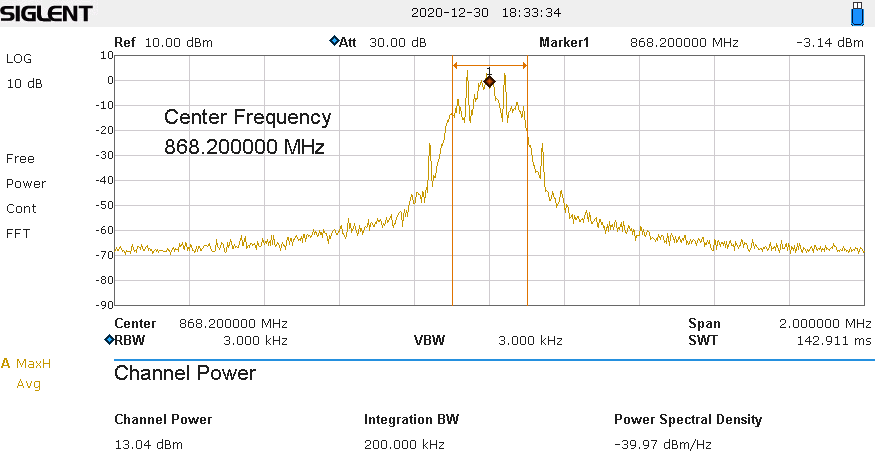
\includegraphics[scale=.5]{spectrum.png}
\caption{Transmit Spectrum of the T-Bone rev.\/1.1 Modem, used in astir13/SoftRF HW rev.\/1.0}\label{spectrum}
\end{figure}\FloatBarrier


\subsection{General Data}
Applicable for use with the "Legacy" protocol (compatible with Flarm v6):

\begin{tabular}{r|c|p{6cm}}\hline
Item & Value & Unit\\\hline\hline
Supply Voltage & 8-20 & V\\\hline
typical supply current & 100 & mA\\\hline
maximum supply current & 300 & mA  \\\hline
weight & 250 & g (including battery, antenna, power switch, cabling and Flarm LED)\\\hline
ambient temperature range & 0 - 40 & $^\circ$C \\\hline
battery type & 18650 Li-Ion & with protection\\
battery voltage typ. & 3.7 & V\\
max. & 4.2 & V\\
min. protection shut off & 3.1 & V\\\hline
channel bandwidth & 125 & kHz\\
modulation type & 2-FSK & \\
bitrate & 100 & kbps\\
max. transmit power & +14 & dBm in "EU" setting\\
 & +17 & dBm in "FULL" setting\\
 & +3 & dBm in "LOW" setting\\
max. transmit duty cycle & $< 1$ & \%\\
transmit frequency stability & +/-15 & kHz\\\hline
GNSS chipset & uBlox NEO6M & \\\hline

\end{tabular}

\section{License}
Copyright (C)  2020-2021 Stefan Pielmeier (sp@symlinux.com)\\

\begin{center}
\fbox{\parbox{12cm}{Permission is granted to copy, distribute and/or modify this document
    under the terms of the GNU Free Documentation License, Version 1.3
    or any later version published by the Free Software Foundation;
    with no Invariant Sections, no Front-Cover Texts, and no Back-Cover Texts.
    A copy of the license is included in the section entitled "GNU
    Free Documentation License".}}
\end{center}    
\end{document}